\section{Introduction}
\begin{comment}
- find better motivation on how much impact the tone of conversation have on SE success
- give existing and future works that we can perform by analyzing the texts
- give more details on how previous studies have inaccurate results 
\end{comment}
% Dr. e wanted a better motivation. Here it is.
Mental state of a person, or simply "mood", affects various different activities like creativity, memory tasks, reasoning, behavior, information processing, learning and decision making~\cite{khan2011moods}. Hence, it influences one's
activities and performance. Khan and his colleagues shows that this also applies to programmers as programming involves different forms of cognitive tasks~\cite{khan2011moods}. The collaborative nature of today's software development makes it an even more vital issue as it requires (significant) human interaction, which subsequently can play a role in determining the mood of an individual, or an entire group  ~\cite{murgia2014developers,graziotin2014happy,curtis1988field}. Study in other domains also show that organizational events can cause affective reactions which in turn influence performance and job satisfaction ~\cite{parkinson1996changing}.

The study of emotional awareness in software engineering therefore has seen a rise in recent years ~\cite{jongeling2017negative}. These studies involve mining software artifacts, understanding the signs of human emotions hidden in them, and the capture and analysis of these data in automated ways. The results and findings can be used in better tracking of the mood in a software team and formulating new strategies to ensure a healthy environment. (These works will come in related work)

Software engineers today have a greater use of using social media to communicate with each other and web platforms to maintain their projects collaboratively ~\cite{storey2010impact}. As a result, we not only get the detail history of the project build up, but also the associated communication that happens alongside them. This presents the opportunity of using natural language processing tools to do different affect analysis
for different purposes. Apart from doing the sentiment analysis, which is the most common technique to mine opinions and emotions, other techniques such as measuring politeness, or even other narrowly defined emotion such as "love" or "anger" ~\cite{ortu2015bullies}. However, while sentiment analysis is the most established techniques among those, politeness is also a very relevant factor in social collaboration ~\cite{steinmacher2015social}. Hence, we concentrate our focus on these two in this work.

However, using automated tools to rate sentiment and politeness in a text is a challenging task ~\cite{montoyo2012subjectivity}. The first challenge lies in correctly defining the rules on how to annotate texts for these ratings as even human raters find it difficult across different topics ~\cite{wiebe2005annotating}. Also, domain-dependency of such tools is a known problem ~\cite{novielli2015challenges,gamon2005pulse}. And the frequently used tools being trained on domains that are not software engineering related doesn't help either. Applying tools that are trained and tested for unrelated corpus in software engineering domain can lead to inaccurate results ~\cite{jongeling2017negative,ahmed2017senticr}.Hence, an evaluation of any technique of sentiment and politeness analysis should be performed first on a new domain to determine if we can use them reliably for future analyses.  

In our study, we choose GitHub to mine data from which has become the largest code host in the world due to its support for distributed version control and pull-based development ~\cite{gousios2014lean}. Developers have many ways to interact with each other in the platform, and detail history of those conversations get archived. These textual artifacts gives us an opportunity to study the emotional environment within the project and its impact on the overall efficiency of the development process. But in the beginning, we need to evaluate if we can do affect analysis reliably on these textual discussions in GitHub. To achieve that, we randomly chose comments from the pull request review and issue section, and manually annotate 590 comments on their sentiment and politeness rating. We then use this data to evaluate how existing tools perform on GitHub comments. Our study also tries to observe the challenges and possibilities that lie in the way of achieving higher correctness.
\newline
\newline
The major contributions of this paper are (does it need re-ordering?)-
\begin{enumerate}
    \item Ground truth data set of GitHub comments on their sentiment and politeness rating.
    \item An annotation scheme to rate politeness of the discussion texts in collaborative platforms.
    \item Verify one tool each for sentiment and politeness analysis over GitHub comments as acceptable (not sure)
    \item discussion on the challenges of sentiment and politeness analysis in SE domain
\end{enumerate}




\section{Related Work}
%-- give evidence of infinite dimensions of emotions-- not needed
%-- why is github an important domain to look at
\subsection{Sentiment Analysis}\label{rwsent}
Closely connected to Affective Computing, a sizable number of papers that mentions "sentiment analysis" focus on the application of classifying texts as to their polarity (positive, negative or neutral) ~\cite{pang2008opinion}. The concept of identifying polarity of texts originally comes from the attempt to extract the mood of users' when they are giving reviews about movie, restaurant or any news item over online platforms. Eventually, many different domains have also used sentiment analysis with software engineering being no exception to that. Using data from GitHub, Guzman et al. applied this technique to study commit comments ~\cite{guzman2014sentiment}, while Pletea and colleagues tried to find correlation between security related discussions and fluctuating sentiments ~\cite{pletea2014security}. Other platforms, including the gentoo community and Stackoverflow, have also been studied to understand the role of developers’ sentiments in the process of software engineering ~\cite{garcia2013role,islam2016towards,guzman2013towards,novielli2014towards}.

While most of these tools used the existing ones that are used commonly in other domains, Research on specialized tools for software engineering domain is also going on ~\cite{jongeling2017negative,ahmed2017senticr}. This tools try to recover some of the problems of the common sentiment analysis tools that were trained on texts from unrelated domains by having their own sentiment oracle for the SE domain, consisting of StackOverflow comments or code review comments, and using that as a training set for their tools. However, they have used different or no coding rubrics while annotating the texts by human raters, which might lead them in having subtle differences in their understanding of sentiment in SE domain.

\subsection{Politeness Analysis}

Politeness can be described as "the practical application of good manners or etiquette" ~\cite{wiki:pol}. Politeness in manner and conversation is a strong factor in social collaborations ~\cite{ortu2015would,wang2008politeness}. Research is also going on in software engineering domain to study the impact of politeness expressed by the developers on the overall process of software development. For example, Ortu et al. concluded that "the more polite developers were, the less time it took to fix an issue", while Jason and colleagues studied GitHub discussions and found that, "the level of a submitter's prior interaction on a project changed how politely developers discussed the contribution and the nature of proposed alternative solutions"~\cite{ortu2015would,tsay2014let}. However, similar to sentiment analysis, different studies had different method to rate politeness ~\cite{tsay2014let,brownsoftware}.


\subsection{Challenges}

A lot of work can still be done to study the emotional awareness in collaborative software engineering ~\cite{dewan2015towards}. However challenges lie in correctly identifying any type of affect before we can use the data for further analysis.In his work, Murgia explores the possibilities of correctly judging emotions from texts extracted from software engineering platforms ~\cite{murgia2014developers}. He found poor to moderate agreements between human raters on different type of emotions and when more contextual details are provided, human raters sometimes find it confusing to correctly interpret emotions rather than being more confident about it. He concludes that "More investigation is needed before building a fully automatic emotion mining tool".

Another work that explores this difficulty ~\cite{novielli2015challenges}, points towards the domain dependency of existing tools which makes it harder to apply them in new corpora. The paper of Jongeling and his colleagues have shown how different tools lead to different results of sentiment in new data set of SE domain (StackOverflow posts) ~\cite{jongeling2017negative}. They also show that, "this disagreement(between different tools) can lead to diverging conclusions and that previously published results cannot be replicated when different sentiment analysis tools are used." Another work also used existing tools on code review comments from the projects using Gerrit and found poor results ~\cite{ahmed2017senticr}. This establishes that reliability of a tool needs to be proven first, before the result of the tool can be used in any further analyses.
\newline
\newline
Under these contexts, \textit{we do similar evaluation of selected tools on pull request review and issue comments from GitHub, with an addition of politeness analysis. We also try to develop the coding guideline on how to rate these texts based on their sentiment and politeness content. To the best of our knowledge, no other studies have explored GitHub comments from the aspect of this paper.}
   



\section{Methodology}
\subsection{Research Questions}
Our goal in this paper is to evaluate the performance of popular sentiment and politeness analysis tools as we have already mentioned why they are important in software engineering research and why the reliability of the tools' result is a major issue while using their results in further analyses. With that objective, we want to test these tools over a new data set of pull request review and issue comments extracted from real-life GitHub projects. These comments mark interactive discussion between different developers and hence can be the gateway to understand the emotional environment of a project, and how different developers are getting along with each other during the process. 

Sentiment analysis being an active field of research in the past decade and also possessing commercial interest, there are a lot of tools available which rates a text based on its emotional polarity. Jongeling et. al point out four tools as the most commonly used for sentiment analysis across all the domains, as well as software engineering ( SentiStrength, NLTK, Alchemy, Stanford NLP). Although, it excludes tools that are commercial and that require training before they can be applied to labelling new data; but for the same reason they are rarely found to be in use in software engineering research too. We also take another tool from a recent paper, Senti4SD ~\cite{calefato2017sentiment}, into consideration as it is claimed to be “specifically trained to support sentiment analysis in developers’ communication channels”. We select these 5 tools as popular sentiment analysis tools and try to determine if they give satisfactory results on GitHub comments. This leads to our first research question,
\newline
\newline
\textbf{RQ1 - How do popular sentiment analysis tools fare on real-life GitHub comments?}
\newline
\newline
Danescu-Niculescu-Mizil et. al have developed a politeness measurement tool based on requests made in Wikipedia and Stack-Exchange~\cite{danescu2013computational}. In their data, requests from Wikipedia are mainly for edit and other administrative functions, while the requests made in Stack-exchange center around diverse range of topics. Ortu et. al have used this tool in the domain of Software Engineering later on~\cite{ortu2015would}. Another using this tool, another study has shown that sentiment and politeness are independent metrics having weak correlation between them ~\cite{ortu2015bullies}. Based on the relevance of the initial dataset with GitHub pull request comments, and it’s subsequent use in Software Engineering research, we are motivated in testing it’s performance on GitHub as well. Thus leading us to our second research question,
\newline
\newline
\textbf{RQ2: How does popular politeness analysis tool fare on real-life GitHub comments? }
\newline
\newline
\subsection{Tool Description}

\textbf{SentiStrength:} We use a free version of SentiStrength developed by Thelwall et. al ~\cite{thelwall2010sentiment}. The tool has been frequently used in software engineering research ~\cite{garcia2013role,guzman2014sentiment,novielli2015challenges,guzman2013towards} in recent studies. SentiStrength assigns an integer value between 1 to 5 for positive sentiment and -1 to -5 for negative sentiment. We add both the rating for a text, and identify under "positive" sentiment if the sum is greater than zero, "negative" is less than zero and "neutral" otherwise. This interpretation was followed in Jongeling's work ~\cite{jongeling2017negative}.

\textbf{Alchemy:} Alchemy provides a text-processing API which returns a label for sentiment (positive/neutral/negative) for each text with score between -1 to +1 with 0 being neutral, +1 being most positive and -1 being most negative.

\textbf{NLTK:} NLTK~\cite{bird2009natural} has also been used in previous works in the SE domain ~\cite{pletea2014security,rousinopoulos2014sentiment}. We use an API provided in \href{www.text-processing.com}{www.text-processing.com} to get the sentiment analysis. For each text fragment, it returns a label (positive/neutral/negative) with a score between 0 to 1 for each of the 3 categories with 1 being its highest intensity.

\textbf{Stanford NLP:} Stanford NLP divides the text into sentences, and perform a more advanced grammatical evaluation on each sentences by generating sentiment treebank through Recursive Neural Tensor Network ~\cite{socher2013recursive}. It returns an integer score for each sentence (0 for neutral, 1 for positive, -1 for negative) indicating its sentiment label. We rate a text under "positive" or "negative" based on the category that has greater number of sentences and "neutral" otherwise. This approach is taken in similar alignment to the approach taken for SentiStrength.

\textbf{Senti4SD:} This tool is a result of a recent paper~\cite{calefato2017sentiment} which also does a ternary classification of each text by labelling their sentiment as positive, negative or neutral. The tool was build from scratch using questions, answers and comments from StackOverflow as its ground truth. Hence it has the claim to be of closer relevance to Software Engineering domain in its efficiency.

\textbf{Politeness tool:} This tool~\cite{danescu2013computational} tries to measure politeness based on "domain-independent lexical and syntactic features operationalizing key components of politeness theory, such as indirection, deference, impersonalization and modality". It was trained and tested on different corpora and hence has the claim to be domain independent. It returns a politeness score between 0 to 1 for each texts with 1 being the most polite.

\subsection{Data Collection \& Manual Raters}\label{data}

In order to test the performance of our tools, we needed a test data set of manually labeled comments extracted from real life GitHub projects. There are many ways for a developer to put comments in GitHub, e.g. commit comments, comments in pull request review and issue discussion boards. However, while commit comments may contain texts for documentation purpose; pull request review and issue comments are mostly discussion between developers. Hence, the later is a more standard metric of interaction between developers. In our study, we only evaluate comments from pull request review and issue section in GitHub.

To get the comments, we make use of the GHTorrent project\footnote{http://ghtorrent.org/} which maintains a queriable archive of GitHub projects (put year?). However, the data from ghtorrent doesn't contain all the discussion comments under issue section. Also, many comments in GitHub contains code snippets. To remove those, we need the HTML tags around the highlighted portion for detection. For that purpose, we also use web-scrapping method to acquire the comments from the issue section and pull request review comments that are not specific any line/lines of code. This way, we can also get the HTML tags. (rewrite with Justin)

We randomly picked 640 comments from the data we gathered. The rationale behind this was that we need two human coders to manually go through and annotate each comment, as previous study found that, "having more than two raters does not change the agreement significantly" ~\cite{murgia2014developers}. We estimated that 100 comments would take an hour to complete the annotation. We had the author to annotate all the comments and two other coders to separately go through half of the whole comments. 3 hours to annotate 300 comments and 1 hour to go through the annotation schemes and initial examples- 4 hours in total for each of the second and third coder was a reasonable time to ask from them. We took 40 comments extra with the estimated 600 comments, as some comments might turn out invalid during the pre-processing. 
During pre-inspection, we had to remove 50 comments as they were either broken, duplicate, contains only code snippets, non-English or the web URL of the page where the comment is located is currently invalid. The rationale is behind the last reason is that if the coder wants to see the whole discussion of which a comment is a part of to have an understanding of the underlying context, he wouldn't be able to do so as the link is broken. We provide the final 590 comments to the human coders removing only the HTML tags. However, before feeding these comments to the tools, we also remove the code snippets and URLs, as they would get incorrectly processed by the tool wrongly considering them as English texts and hence biasing the result. 

The manual raters involved in our study were graduate and undergraduate students of Computer Science department. We gave a coding guideline to the raters before providing the comments, explained in \ref{sentscheme}, \ref{polscheme}. We also gave a short sample consisting 10 examples to practice before jumping into the main data set. After the first iteration, the author sat with each of the coders to discuss about the comments that were disagreed. The whole process is explained in more detail in \ref{gt}.

\subsection{Sentiment Labelling Annotation}\label{sentscheme}

As mentioned in \ref{rwsent}, previous works have used different or no coding guidelines while doing sentiment rating in SE domain. To not deviate a lot from the previous works, but still giving our coders a basic set of strategies, we make use of the simple annotation scheme developed by Mohammad~\cite{mohammad2016practical} to provide the human raters a basic guideline\footnote{put scheme here}. Based on this scheme, the raters were asked to label each comment as either positive, negative, neutral, mixed or sarcasm. The "mixed" here stand for a text containing both type of emotions. Our tools label texts as "neutral" where opposite emotions counter each other. From that perspective, we eventually classified the texts as "neutral" which were given a "mixed" rating by the human raters. We omitted the texts rated "sarcasm" as there is no clear guideline on how to match its label with the possible ratings the tools has as output.

\subsection{Politeness Labelling Annotation}\label{polscheme}

We could not find any commonly used politeness scheme to rate textual documents. So, we developed and began with an experimental coding scheme based on the work of Brown \& Levinson's politeness theory ~\cite{brown1987politeness} and Culpeper's work of impoliteness
We developed a politeness annotation scheme based on the work of Brown \& Levinson’s politeness theory [16] and Culpeper’s work of impoliteness ~\cite{culpeper1996towards}. (((The scheme also aligns with the findings of Danescu-Niculescu-Mizil et al’s finding of politeness markers in their work [5].))) Our coding scheme depends on four major criteria shown in table 1. Each having subset of rules and examples along with them. put a table here,

However the raters were also asked to use their own judgment, and if they used any other judgment criteria that was not covered in this scheme, put that as an additional remark during rating.

Based on our scheme, raters were asked to rate each text on an integer scale of -2 to +2 with -2 being most impolite, 0 being neutral and +2 being most polite. However, our initial coding was not very clear on how to distinguish between the degree of politeness/impoliteness, hence we got varying judgment about the degree. For the purpose of this study, we therefore merged “very polite” and “polite” into one single group of “polite” and “very impolite” and impolite” into one group of “impolite. (is this a good argument/ explanation?) \footnote{add politeness scheme}


\section{Results}

\subsection{Ground Truth}\label{gt}
We collected annotation from individual raters and built our first set of ground truth based only on those data that had the same label from both the raters. This resulted in 374 comments as ground truth for politeness rating and 285 comments as ground truth for sentiment rating. These comments were eventually used as test data for the evaluation of our tools. The amount of test data is comparable with previous study which took 265 texts of labelled data to perform the evaluation of sentiment analysis tools ~\cite{jongeling2017negative}.

All of the initial 590 comments were annotated by the author, and two other coders annotated half of the dataset each. Table 1 shows the inter-rater agreement. We used Weighted Cohen's Kappa as our classes in both the ratings have an implicit ordering. When two coder labelled different polarity for both the ratings (“positive” vs “negative” and “polite” vs “impolite”), we counted it as a strong disagreement (weight=2). And when one of the labels was “neutral”, and other was a polar one, we counted it as a weak disagreement (weight=1).

Table 1 shows agreement rate between author and both the coders. The Author’s ratings fared “fair” and “moderate” agreement with Coder 1 in sentiment and politeness respectively and “fair” with Coder 2 in both the ratings (according to magnitude guidelines presented by Landis and Koch~\cite{landis1977measurement}). The “unsubstantial” agreement between the raters points towards the subjectivity of the matter. Another reason can be the difficulty in understanding proper context in the domain discussed in an earlier work[24].
How many pos, neg and neutral? give agreement rating of previous papers
how many polite, impolite and neutral
\begin{table}
  \caption{Agreement rate among manual Raters}
  \label{tab:freq}
  \begin{tabular}{|c|c|l|}
    \toprule
    Weighted K & Author and Coder 1 &  Author and  Coder 2\\
    \midrule
    Sentiment & .38 & .27 \\
    \hline
    Politeness & .48 & .36\\
  \bottomrule
\end{tabular}
\end{table}

The author then sat with each of the other coder to discuss about the disagreed comments. Then upon discussion, the raters came for a final rating for all of the comments. now pos was , neg was and neu. similarly pol, neu and impolite was . The raters also discussed the reason behind choosing the final rating for them and how the annotation scheme should be modified or added to improve.
\subsection{RQ1}

198 out of total 285 comments being “neutral” in our ground truth for sentiment analysis, only F-measures for the tools would be a misleading metric as the agreement by chance would be pretty high. So, we also calculated Weighted Cohen’s Kappa as before, to compare the tools. Apart from the 5 selected tools, we also considered an aggregated method of these tools which considers the majority voting criteria to give its result, and included its performance with others.
From the results in Table 2, Senti4SD turned out to have the best performance among the tools. Also the moderate agreement rate, .53, which is even better than mutual agreements between the human coders, shows that the tool has acceptable performance over GitHub comments.
One interesting aspect, however, is the bad performance over negative comments by all the tools. Unlike positive and neutral comments, it can be argued if we can justify any of the tools’ result on “negative” sentiment of the comments as reliable.
negative bias also in previous papers results. 
\begin{tabular}{ccccc}
& & & & \\
\multicolumn{2}{c}{ } & \multicolumn{3}{c}{ F-measure } \\
tools & k & neu & pos & neg \\
SentiStrength & 0.44 & 74.58\% & 61.54\% & 40.68\% \\
NLTK & 0.27 & 52.63\% & 55.42\% & 23.73\% \\
Alchemy & 0.33 & 58.78\% & 58.21\% & 32.65\% \\
Stanford NLP & 0.26 & 55.85\% & 59.83\% & 19.44\% \\
Senti4SD & 0.53 & 84.92\% & 68.18\% & 41.03\% \\
\end{tabular}

Give result with all of the comments.

\begin{tabular}{ccccc}
& & & & \\
\multicolumn{2}{c}{ } & \multicolumn{3}{c}{ F-measure } \\
tools & k & neu & pos & neg \\
SentiStrength & 0.44 & 74.58\% & 61.54\% & 40.68\% \\
NLTK & 0.27 & 52.63\% & 55.42\% & 23.73\% \\
Alchemy & 0.33 & 58.78\% & 58.21\% & 32.65\% \\
Stanford NLP & 0.26 & 55.85\% & 59.83\% & 19.44\% \\
Senti4SD & 0.53
\end{tabular}

\subsection{RQ2}

As our politeness tool gives a rating between 0 to 1 for each texts for its politeness, we have to first select a bar where we can separate the polite, impolite and neutral comments.
We calculated F-measures at every .01 interval within the 0-1 range. We found highest F-measure being 69.61\%  for “polite” at .57 bar and 77.05\% for “neutral” at .65 bar. So, intuitively the ideal bar would fall somewhere between that range. Our results align with the findings of Jongeling et. al, who found this bar to be at .611 over their dataset in software engineering domain. So, we use this bar and rate all those comments as “polite” for which the tool gives a higher rating than .611.
However, we found very poor result for “impolite” comments as F-measures at all the bars were below 20\%. Thus, we concluded that it is not possible to use the tool to reliably label a text as “impolite”.
From this conclusion, we decided to merge the “neutral” and “impolite” class into one single class that is “non-polite”. Thus, eventually we use the tool for a binary classification of the texts between “polite” and “non-polite”.
We use our ground-truth dataset of 374 comments for politeness rating to test this tool. Similar to RQ1, we use cohen’s kappa (unweighted) and F-measures as our metrics.
Table 3 shows that this tool also has “moderate” agreement rate which is also better than what our human coders had between themselves. The performance hence can be taken as acceptable over GitHub comments.

\begin{tabular}{cc}
& \\
\multicolumn{2}{c}{ F-measure } \\
polite & neutral \\
67.15 & 75.94 \\
& \\
\end{tabular}

give rating over all of the comments 

\begin{tabular}{cc}
& \\
\multicolumn{2}{c}{ F-measure } \\
polite & neutral \\
67.15 & 75.94 \\
& \\
\end{tabular}
one threat to validity is that our coding guideline align with the tools strategies. 
\subsection{Final Politeness Annotation Scheme}

Based on the discussion, we adjusted few points here and there about the annotation scheme and made a complete scheme. describe.

\subsection{ MOdified Sentiment Annotation Scheme}

we added some rules to remove vagueness from the initial scheme which was much broader in general.

\section{Discussion}

Sentiment and Politeness both are highly subjective topics. The low agreement rates between the human coders on sentiment make us question about the overall authenticity of doing sentiment analysis in Software Engineering domain. This technique is used in movie and sports reviews or news items to mine people's opinion as they often offer their judgement on different matters explicitly or implicitly. However, in platforms like GitHub, the discussions are less filled with human emotions, and are rather direct work-like discussions on specific program codes or development processes.
	The politeness, however seems to be a more relevant idea in these collaboration platforms. The higher agreement rates between human coders support this intuition. The author’s manual inspection over the comments also gives us the idea that there are certain patterns to express politeness in written comments. These patterns are well-aligned with the common politeness theories in linguistic studies. We tried to build an annotation scheme to mark politeness in such written texts. More iteration and modification is needed before it can be used as a gold standard. For the improvement of the tools’ performances, a domain based training is helpful whatsoever.  
	One interesting observation is that, “positive” sentiments were often correlated with “politeness” in our manually labelled data. Aggregating the two techniques may give even better results in politeness rating. However, a larger dataset is required to verify this claim. The failure in detecting the opposite extremes, “negative” and “impolite” comments, also gives us foods for thought.
In conclusion, despite the high subjectivity of the topics, we verified two tools to give acceptable results in  identifying “positive” and “polite” comments. To count the impact of such comments over different aspects in future, one can reliably use these tools in practice.



\begin{comment}
\subsection{Citations}
Citations to articles~\cite{bowman:reasoning,
clark:pct, braams:babel, herlihy:methodology},
conference proceedings~\cite{clark:pct} or maybe
books \cite{Lamport:LaTeX, salas:calculus} listed
in the Bibliography section of your
article will occur throughout the text of your article.
You should use BibTeX to automatically produce this bibliography;
you simply need to insert one of several citation commands with
a key of the item cited in the proper location in
the \texttt{.tex} file~\cite{Lamport:LaTeX}.
The key is a short reference you invent to uniquely
identify each work; in this sample document, the key is
the first author's surname and a
word from the title.  This identifying key is included
with each item in the \texttt{.bib} file for your article.

The details of the construction of the \texttt{.bib} file
are beyond the scope of this sample document, but more
information can be found in the \textit{Author's Guide},
and exhaustive details in the \textit{\LaTeX\ User's
Guide} by Lamport~\shortcite{Lamport:LaTeX}.

This article shows only the plainest form
of the citation command, using \texttt{{\char'134}cite}.

Some examples.  A paginated journal article \cite{Abril07}, an enumerated
journal article \cite{Cohen07}, a reference to an entire issue \cite{JCohen96},
a monograph (whole book) \cite{Kosiur01}, a monograph/whole book in a series (see 2a in spec. document)
\cite{Harel79}, a divisible-book such as an anthology or compilation \cite{Editor00}
followed by the same example, however we only output the series if the volume number is given
\cite{Editor00a} (so Editor00a's series should NOT be present since it has no vol. no.),
a chapter in a divisible book \cite{Spector90}, a chapter in a divisible book
in a series \cite{Douglass98}, a multi-volume work as book \cite{Knuth97},
an article in a proceedings (of a conference, symposium, workshop for example)
(paginated proceedings article) \cite{Andler79}, a proceedings article
with all possible elements \cite{Smith10}, an example of an enumerated
proceedings article \cite{VanGundy07},
an informally published work \cite{Harel78}, a doctoral dissertation \cite{Clarkson85},
a master's thesis: \cite{anisi03}, an online document / world wide web
resource \cite{Thornburg01, Ablamowicz07, Poker06}, a video game (Case 1) \cite{Obama08} and (Case 2) \cite{Novak03}
and \cite{Lee05} and (Case 3) a patent \cite{JoeScientist001},
work accepted for publication \cite{rous08}, 'YYYYb'-test for prolific author
\cite{SaeediMEJ10} and \cite{SaeediJETC10}. Other cites might contain
'duplicate' DOI and URLs (some SIAM articles) \cite{Kirschmer:2010:AEI:1958016.1958018}.
Boris / Barbara Beeton: multi-volume works as books
\cite{MR781536} and \cite{MR781537}.

A couple of citations with DOIs: \cite{2004:ITE:1009386.1010128,
  Kirschmer:2010:AEI:1958016.1958018}.

Online citations: \cite{TUGInstmem, Thornburg01, CTANacmart}.


\subsection{Tables}
Because tables cannot be split across pages, the best
placement for them is typically the top of the page
nearest their initial cite.  To
ensure this proper ``floating'' placement of tables, use the
environment \textbf{table} to enclose the table's contents and
the table caption.  The contents of the table itself must go
in the \textbf{tabular} environment, to
be aligned properly in rows and columns, with the desired
horizontal and vertical rules.  Again, detailed instructions
on \textbf{tabular} material
are found in the \textit{\LaTeX\ User's Guide}.

Immediately following this sentence is the point at which
Table~\ref{tab:freq} is included in the input file; compare the
placement of the table here with the table in the printed
output of this document.

\begin{table}
  \caption{Frequency of Special Characters}
  \label{tab:freq}
  \begin{tabular}{ccl}
    \toprule
    Non-English or Math&Frequency&Comments\\
    \midrule
    \O & 1 in 1,000& For Swedish names\\
    $\pi$ & 1 in 5& Common in math\\
    \$ & 4 in 5 & Used in business\\
    $\Psi^2_1$ & 1 in 40,000& Unexplained usage\\
  \bottomrule
\end{tabular}
\end{table}

To set a wider table, which takes up the whole width of the page's
live area, use the environment \textbf{table*} to enclose the table's
contents and the table caption.  As with a single-column table, this
wide table will ``float'' to a location deemed more desirable.
Immediately following this sentence is the point at which
Table~\ref{tab:commands} is included in the input file; again, it is
instructive to compare the placement of the table here with the table
in the printed output of this document.


\begin{table*}
  \caption{Some Typical Commands}
  \label{tab:commands}
  \begin{tabular}{ccl}
    \toprule
    Command &A Number & Comments\\
    \midrule
    \texttt{{\char'134}author} & 100& Author \\
    \texttt{{\char'134}table}& 300 & For tables\\
    \texttt{{\char'134}table*}& 400& For wider tables\\
    \bottomrule
  \end{tabular}
\end{table*}
% end the environment with {table*}, NOTE not {table}!

It is strongly recommended to use the package booktabs~\cite{Fear05}
and follow its main principles of typography with respect to tables:
\begin{enumerate}
\item Never, ever use vertical rules.
\item Never use double rules.
\end{enumerate}
It is also a good idea not to overuse horizontal rules.


\subsection{Figures}

Like tables, figures cannot be split across pages; the best placement
for them is typically the top or the bottom of the page nearest their
initial cite.  To ensure this proper ``floating'' placement of
figures, use the environment \textbf{figure} to enclose the figure and
its caption.

This sample document contains examples of \texttt{.eps} files to be
displayable with \LaTeX.  If you work with pdf\LaTeX, use files in the
\texttt{.pdf} format.  Note that most modern \TeX\ systems will convert
\texttt{.eps} to \texttt{.pdf} for you on the fly.  More details on
each of these are found in the \textit{Author's Guide}.

\begin{figure}
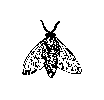
\includegraphics{fly}
\caption{A sample black and white graphic.}
\end{figure}

\begin{figure}
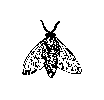
\includegraphics[height=1in, width=1in]{fly}
\caption{A sample black and white graphic
that has been resized with the \texttt{includegraphics} command.}
\end{figure}


As was the case with tables, you may want a figure that spans two
columns.  To do this, and still to ensure proper ``floating''
placement of tables, use the environment \textbf{figure*} to enclose
the figure and its caption.  And don't forget to end the environment
with \textbf{figure*}, not \textbf{figure}!

\begin{figure*}
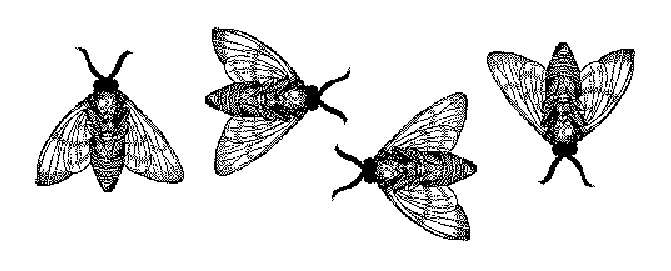
\includegraphics{flies}
\caption{A sample black and white graphic
that needs to span two columns of text.}
\end{figure*}


\begin{figure}
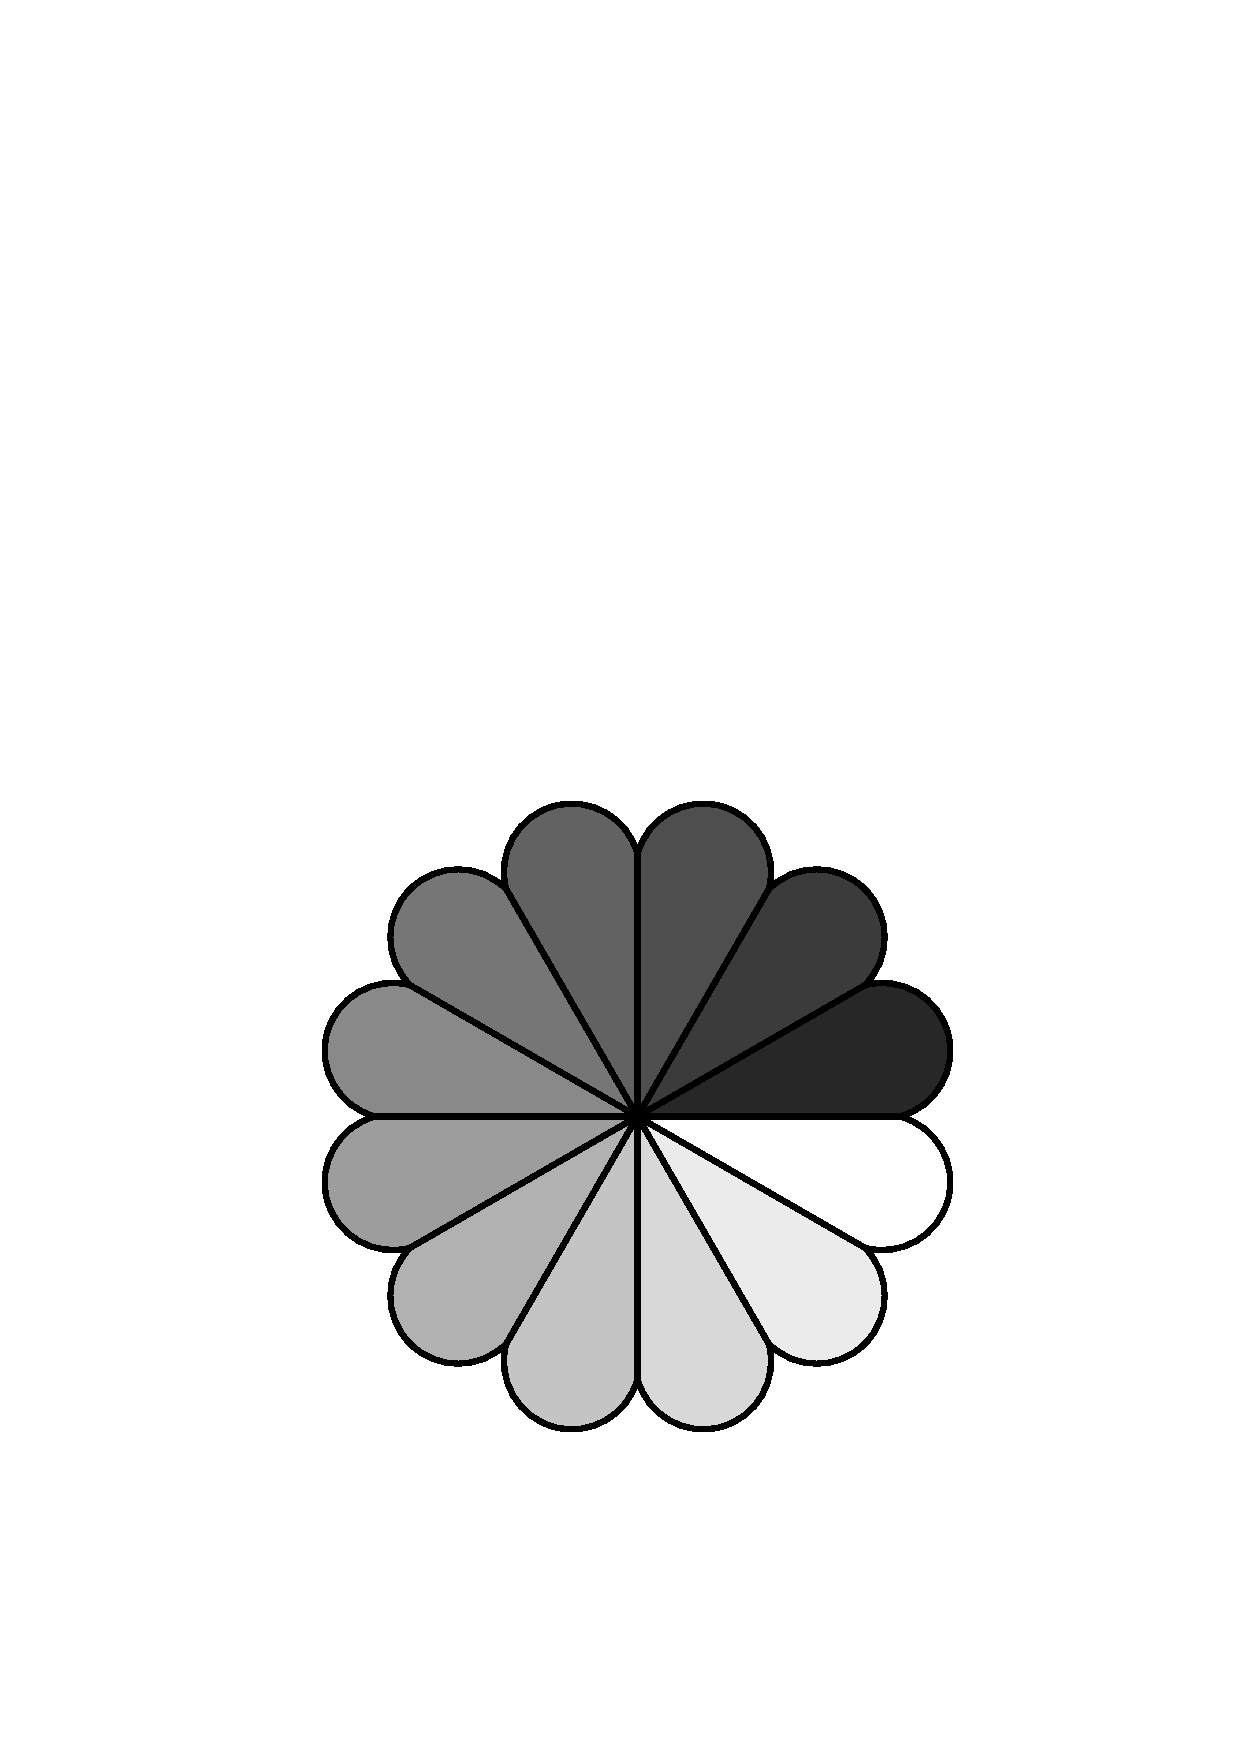
\includegraphics[height=1in, width=1in]{rosette}
\caption{A sample black and white graphic that has
been resized with the \texttt{includegraphics} command.}
\end{figure}

\subsection{Theorem-like Constructs}

Other common constructs that may occur in your article are the forms
for logical constructs like theorems, axioms, corollaries and proofs.
ACM uses two types of these constructs:  theorem-like and
definition-like.

Here is a theorem:
\begin{theorem}
  Let $f$ be continuous on $[a,b]$.  If $G$ is
  an antiderivative for $f$ on $[a,b]$, then
  \begin{displaymath}
    \int^b_af(t)\,dt = G(b) - G(a).
  \end{displaymath}
\end{theorem}

Here is a definition:
\begin{definition}
  If $z$ is irrational, then by $e^z$ we mean the
  unique number that has
  logarithm $z$:
  \begin{displaymath}
    \log e^z = z.
  \end{displaymath}
\end{definition}

The pre-defined theorem-like constructs are \textbf{theorem},
\textbf{conjecture}, \textbf{proposition}, \textbf{lemma} and
\textbf{corollary}.  The pre-defined de\-fi\-ni\-ti\-on-like constructs are
\textbf{example} and \textbf{definition}.  You can add your own
constructs using the \textsl{amsthm} interface~\cite{Amsthm15}.  The
styles used in the \verb|\theoremstyle| command are \textbf{acmplain}
and \textbf{acmdefinition}.

Another construct is \textbf{proof}, for example,

\begin{proof}
  Suppose on the contrary there exists a real number $L$ such that
  \begin{displaymath}
    \lim_{x\rightarrow\infty} \frac{f(x)}{g(x)} = L.
  \end{displaymath}
  Then
  \begin{displaymath}
    l=\lim_{x\rightarrow c} f(x)
    = \lim_{x\rightarrow c}
    \left[ g{x} \cdot \frac{f(x)}{g(x)} \right ]
    = \lim_{x\rightarrow c} g(x) \cdot \lim_{x\rightarrow c}
    \frac{f(x)}{g(x)} = 0\cdot L = 0,
  \end{displaymath}
  which contradicts our assumption that $l\neq 0$.
\end{proof}

\section{Conclusions}
This paragraph will end the body of this sample document.
Remember that you might still have Acknowledgments or
Appendices; brief samples of these
follow.  There is still the Bibliography to deal with; and
we will make a disclaimer about that here: with the exception
of the reference to the \LaTeX\ book, the citations in
this paper are to articles which have nothing to
do with the present subject and are used as
examples only.
%\end{document}  % This is where a 'short' article might terminate



\appendix
%Appendix A
\section{Headings in Appendices}
The rules about hierarchical headings discussed above for
the body of the article are different in the appendices.
In the \textbf{appendix} environment, the command
\textbf{section} is used to
indicate the start of each Appendix, with alphabetic order
designation (i.e., the first is A, the second B, etc.) and
a title (if you include one).  So, if you need
hierarchical structure
\textit{within} an Appendix, start with \textbf{subsection} as the
highest level. Here is an outline of the body of this
document in Appendix-appropriate form:
\subsection{Introduction}
\subsection{The Body of the Paper}
\subsubsection{Type Changes and  Special Characters}
\subsubsection{Math Equations}
\paragraph{Inline (In-text) Equations}
\paragraph{Display Equations}
\subsubsection{Citations}
\subsubsection{Tables}
\subsubsection{Figures}
\subsubsection{Theorem-like Constructs}
\subsubsection*{A Caveat for the \TeX\ Expert}
\subsection{Conclusions}
\subsection{References}
Generated by bibtex from your \texttt{.bib} file.  Run latex,
then bibtex, then latex twice (to resolve references)
to create the \texttt{.bbl} file.  Insert that \texttt{.bbl}
file into the \texttt{.tex} source file and comment out
the command \texttt{{\char'134}thebibliography}.
% This next section command marks the start of
% Appendix B, and does not continue the present hierarchy
\section{More Help for the Hardy}

Of course, reading the source code is always useful.  The file
\path{acmart.pdf} contains both the user guide and the commented
code.

\begin{acks}
  The authors would like to thank Dr. Yuhua Li for providing the
  MATLAB code of the \textit{BEPS} method.

  The authors would also like to thank the anonymous referees for
  their valuable comments and helpful suggestions. The work is
  supported by the \grantsponsor{GS501100001809}{National Natural
    Science Foundation of
    China}{http://dx.doi.org/10.13039/501100001809} under Grant
  No.:~\grantnum{GS501100001809}{61273304}
  and~\grantnum[http://www.nnsf.cn/youngscientists]{GS501100001809}{Young
    Scientists' Support Program}.

\end{acks}
\end{comment}